\begin{figure*}[htp]
  \centering
  \begin{subfigure}[b]{0.475\textwidth}
      \centering
      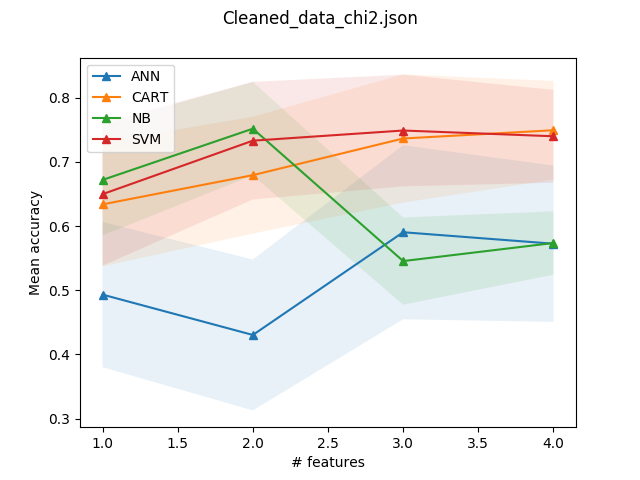
\includegraphics[width=\textwidth]{../plots_with_std_fill/Cleaned_data_chi2_combined.png}
      \caption[]%
      {{\small}}
      \label{fig:EN_chi2}
  \end{subfigure}
  \hfill
  \begin{subfigure}[b]{0.475\textwidth}
      \centering
      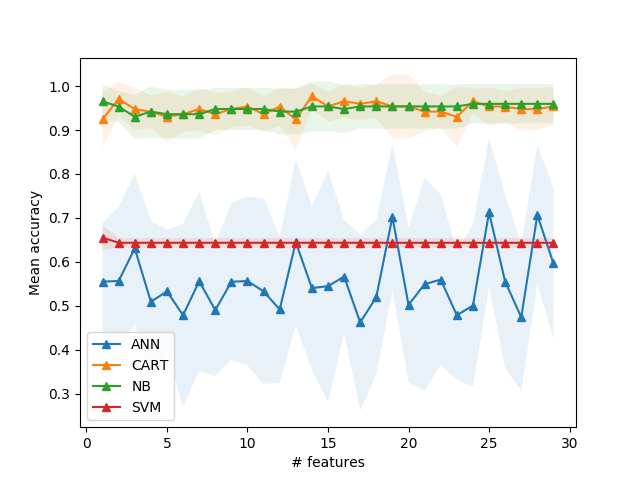
\includegraphics[width=\textwidth]{../plots_with_std_fill/data_FNA_chi2_combined.png}
      \caption[]%
      {{\small}}
      \label{fig:WBCD_chi2}
  \end{subfigure}
  \vskip\baselineskip
  \begin{subfigure}[b]{0.475\textwidth}
      \centering
      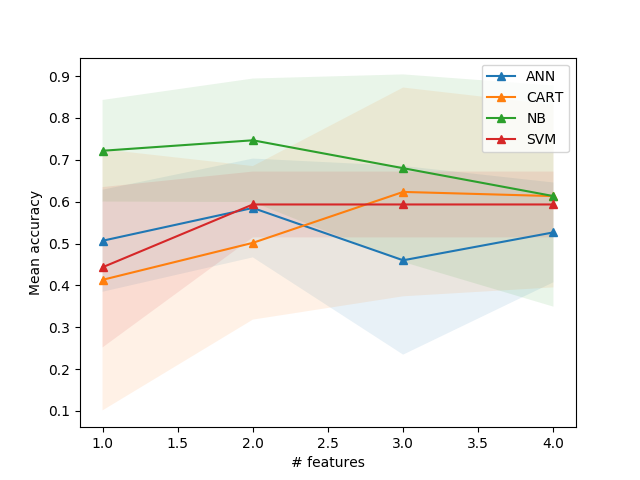
\includegraphics[width=\textwidth]{../plots_with_std_fill/Data_mias_chi2_combined.png}
      \caption[]%
      {{\small}}
      \label{fig:MIAS_chi2}
  \end{subfigure}
  \quad
  \begin{subfigure}[b]{0.475\textwidth}
      \centering
      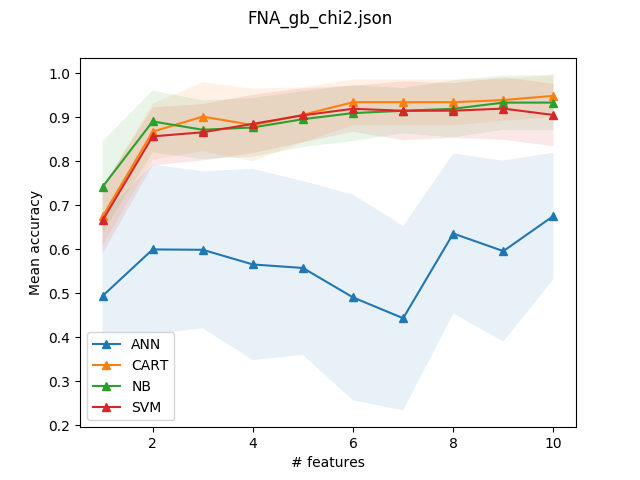
\includegraphics[width=\textwidth]{../plots_with_std_fill/FNA_gb_chi2_combined.png}
      \caption[]%
      {{\small}}
      \label{fig:RHH_chi2}
  \end{subfigure}
  \caption[]
  {\small (a) Dataset EN using Chi2. (b) Dataset WBCD using Chi2. (c) Dataset MIAS using Chi2. (d) Dataset RHH using Chi2.  Combined plots of all datasets comparing each classifier when using chi2 for feature selection.}
  \label{fig:plots_chi2}
\end{figure*}
